\section{A Compact Representation of a Ring of Sets}

In this section, we demonstrate how the marriage lattice $\mathcal{M}$ representation, $I(\mathcal{M})$, can be extended to a general representation $I(\mathcal{F})$ for any ring of sets $\mathcal{F}$. The definitions and proofs in this section are very similar to those used for $I(\mathcal{M})$, although with some minor distinctions.

For any element $a \in B$, we let $\mathcal{F}(a)$ denote the set of all elements of $\mathcal{F}$ that contain $a$. It may happen that $\mathcal{F}(a)$ is empty, but if $F_i$ and $F_j$ belong to $\mathcal{F}(a)$, then so also do $F_i \cup F_j$ and $F_i \cap F_j$ . So $\mathcal{F}(a)$ itself forms a ring of sets over $B$, and there is therefore a \textbf{unique minimal} and a \textbf{unique maximal} element of $\mathcal{F}(a)$; we define $F(a)$ to be the unique \textit{minimal element} of $\mathcal{F}(a)$. That is, $F(a) = \{F : F \in \mathcal{F}(a)\}$. Then, an element $F$ of $\mathcal{F}$ that is $F(a)$ for some $a$ will be called $irreducible$, and we use $I(\mathcal{F})$ to denote the set of all \textit{irreducible elements} of $\mathcal{F}$. We also view $(I(F), \preceq)$ as a partial order under the relation $\preceq$ of set containment: if $F$ and $F^\prime$ are elements of $\mathcal{F}$, then $F$ precedes $F^\prime$ in $(I(F),\preceq)$ if and only if $F \subseteq F^\prime$.

\begin{exmp}\label{exmp_2_5}
 Consider the ring of sets $\mathcal{F}$ displayed by the \textit{Hasse diagram} of $\mathcal{F}$ in Figure \ref{FIG_2_5}. The base of this ring is the set $\{a, b, c, d, e, f, g, h, i\}$, and there is an edge from a set $F$ to a set $F^\prime$ if and only if $F$ is an immediate predecessor of $F^\prime$, i.e., $F \subset F^\prime$, and there is no set $F^{\prime \prime}$ such that $F \subset F^{\prime \prime} \subset F^\prime$. The \textit{irreducible} elements of the ring are $\{F_0, F_1, F_2, F_3, F_5, F_{11}\}$, and each such $F$ is $F(x)$ for every underlined element $x$ in $F$, i.e., $F$ is the minimal element of $\mathcal{F}$ containing $x \in B$. The partial order $I(\mathcal{F})$ is shown in Figure \ref{FIG_2_6}
\end{exmp}

\begin{figure}[ht]
  \centering
  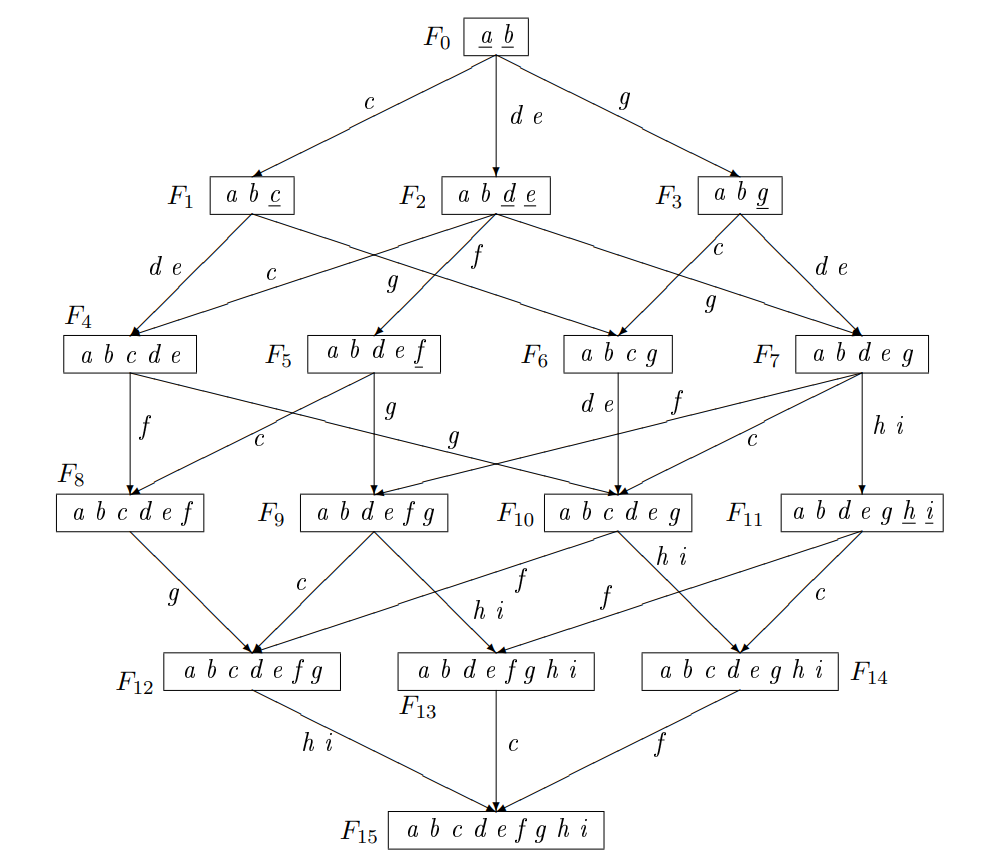
\includegraphics[width=1\textwidth]{IMAGES_FIGS/FIG_2_4.png}
  \caption{A ring of sets with $B = \{a, b, c, d, e, f, g, h, i\}$}
  \label{FIG_2_5}
\end{figure}

\begin{figure}[ht]
  \centering
  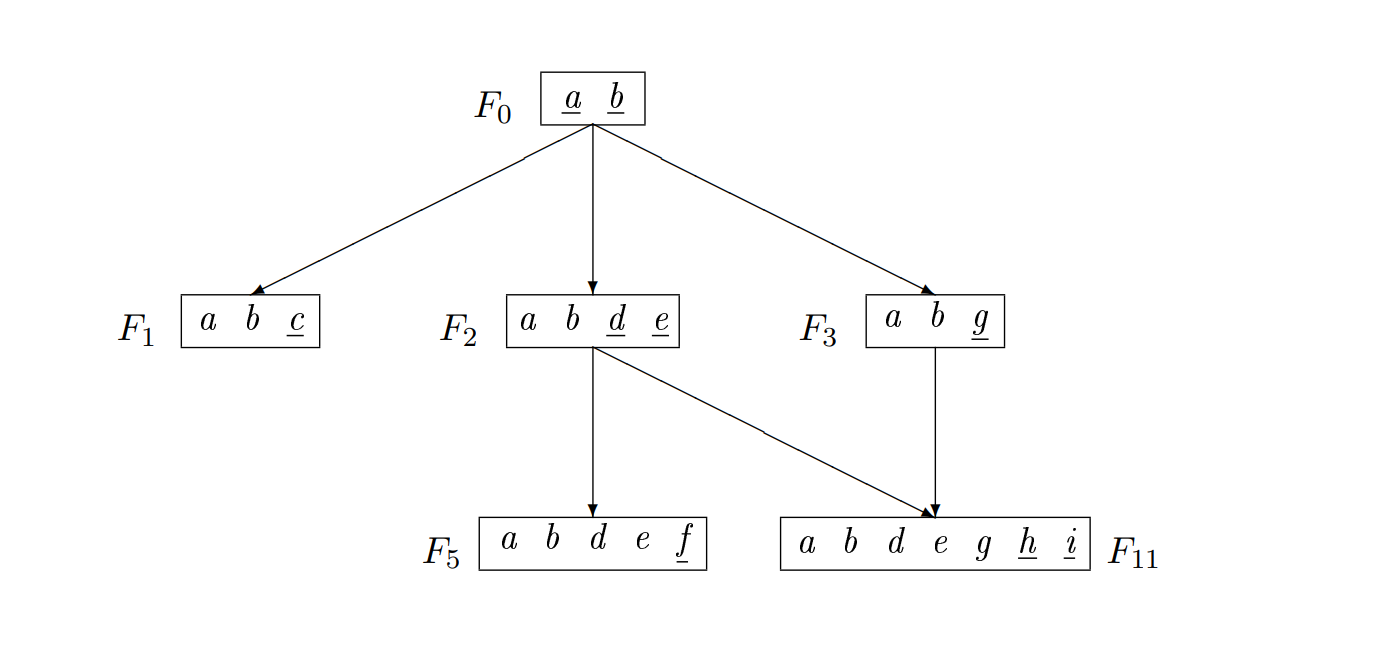
\includegraphics[width=0.85\textwidth]{IMAGES_FIGS/FIG_2_5.png}
  \caption{The partial order $I(\mathcal{F})$ of the irreducible elements of $\mathcal{F}$}
  \label{FIG_2_6}
\end{figure}

Let $S$ be any nonempty subset of $I(\mathcal{F})$. Since $\mathcal{F}$ is closed under \textit{union}, $\cup\{F : F \in S\}$ is a subset of B that is in $\mathcal{F}$. Hence each nonempty closed subset of $I(\mathcal{F})$ generates an element of $\mathcal{F}$ in this way. Our immediate objective is to show that this correspondence between nonempty closed subsets of $I(\mathcal{F})$ and elements of $\mathcal{F}$ is one-one.

For an arbitrary element $F$ of $\mathcal{F}$, we define the irreducible support $U(F)$ of $F$ to be $\{F(a): a \in$ $F\}$

\begin{lemma}\label{lem_2_4}
For any element $F$ of $\mathcal{F}$, the irreducible support of $F$ is closed in $I(\mathcal{F})$. Equivalently, $U(F)$ is the set of all irreducible elements of $\mathcal{F}$ that precede $F$ in $\mathcal{F}$, i.e., that are subsets of $F$.
\end{lemma}

\begin{proof}
Let $F_1 \subset F_2$ be two distinct irreducible elements of $\mathcal{F}$, and let $F_2$ be in $U(F)$. We will show that $F_1$ is in $U(F)$. Since $F_1$ is irreducible, $F_1=F(b)$ for some $b \in B$. Similarly, $F_2=F(a)$ for some $a \in F$, so $b$ must be in $F(a)$. Now $a \in F$ implies that $F(a) \subseteq F$, so it follows that $b$ is in $F$, and hence $F(b)$, which is $F_1$, is in $U(F)$.
\end{proof}

\begin{exmp}\label{exmp_2_6}
    We have $U\left(F_9\right)=\left\{F_0, F_2, F_3, F_5\right\}$, which is indeed closed in $I(\mathcal{F})$, and is the set of all irreducible elements of $\mathcal{F}$ that precede $F_9$ in $\mathcal{F}$. Note that we have not defined any object similar to $\hat{U}$, the closure of $U$, which was defined in the discussion of $I(\mathcal{M})$. The reason is that, unlike $U(F)$, which is closed in $\mathcal{F}, U(M)$ is not always closed for any $M \in \mathcal{M}$.
\end{exmp}

\begin{lemma}\label{lem_2_5}
 For any element $F$ of $\mathcal{F}, F=\cup U(F)$. That is, $F$ can be expressed as the union of its irreducible support.   
\end{lemma}

\begin{proof}
    For any element $a \in F, a$ is in $F(a)$, which is in $U(F)$, so $a$ is in $\cup U(F)$, hence $F \subseteq \cup U(F)$. Conversely, every element of $U(F)$ is a subset of $F$, so $\cup U(F) \subseteq F$.
\end{proof}

\begin{lemma}\label{lem_2_6}
    $F$ is irreducible if and only if $F$ cannot be written as the union of members of $\mathcal{F}$ excluding $F$ itself.
\end{lemma}

\begin{lemma}\label{lem_2_7}
    If $S$ and $T$ are distinct closed subsets of $I(\mathcal{F})$, then $\cup S \neq \cup T$.
\end{lemma}

\begin{proof}
    If $S$ and $T$ are different closed subsets of $I(\mathcal{F})$, then one of them, say $S$, contains an element $F=F(a)$ that is not contained in the other set, $T$. But $F(a)$ is contained in all members of $\mathcal{F}$ that contain $a$, so no such member of $\mathcal{F}$ is in $T$. Hence $a \in \cup S, a \notin \cup T$, and therefore $\cup S \neq \cup T$.
\end{proof}
\newpage
\begin{theo}
So, in summary we have :
\begin{itemize}
    \item There is a one-one correspondence between the elements of $\mathcal{F}$ and the nonempty closed subsets of $I(\mathcal{F})$. In particular, an element $F$ of $\mathcal{F}$ corresponds to $U(F)$, which is a closed subset in $I(\mathcal{F})$.
    \item Each nonempty closed subset of $I(\mathcal{F})$ generates (by unioning) an element of $\mathcal{F}$, and each element of $\mathcal{F}$ is generated in this way by exactly one nonempty closed subset of $I(\mathcal{F})$.
    \item If $S$ and $S^{\prime}$ are closed subsets of $I(\mathcal{F})$ that generate $F$ and $F^{\prime}$ respectively, then $F \subseteq F^{\prime}$ if and only if $S \subseteq S^{\prime}$.
\end{itemize}
\end{theo}

\begin{exmp}\label{exmp_2_7}
    There are sixteen nonempty closed subsets of $I(\mathcal{F})$ each generates a distinct element of $\mathcal{F}$, and each is the irreducible support of that element. Figure \ref{FIG_2_7} shows the elements of $\mathcal{F}$, and for each one, the unique nonempty closed subset of $I(\mathcal{F})$ that generates it.
\end{exmp}

\begin{center}
    $\begin{array}{lllllll}F_0: & F_0 & & & & & \\ F_1: & F_0 & F_1 & & & & \\ F_2: & F_0 & F_2 & & & & \\ F_3: & F_0 & F_3 & & & & \\ F_4: & F_0 & F_1 & F_2 & & & \\ F_5: & F_0 & F_2 & F_5 & & & \\ F_6: & F_0 & F_1 & F_3 & & & \\ F_7: & F_0 & F_2 & F_3 & & & \\ F_8: & F_0 & F_1 & F_2 & F_5 & & \\ F_9: & F_0 & F_2 & F_3 & F_5 & & \\ F_{10}: & F_0 & F_1 & F_2 & F_3 & & \\ F_{11}: & F_0 & F_2 & F_3 & F_{11} & & \\ F_{12}: & F_0 & F_1 & F_2 & F_3 & F_5 & \\ F_{13}: & F_0 & F_2 & F_3 & F_5 & F_{11} & \\ F_{14}: & F_0 & F_1 & F_2 & F_3 & F_{11} & \\ F_{15}: & F_0 & F_1 & F_2 & F_3 & F_5 & F_{11} \end{array}$
    \begin{figure}[ht]
  \centering
  \caption{The elements of $\mathcal{F}$ and their associated closed subsets of $I(\mathcal{F})$}
  \label{FIG_2_7}
\end{figure}
    %REF TO FIGURE
\end{center}

\subsection{$I(\mathcal{F})$ reduces to $I(\mathcal{M})$}
When $\mathcal{F}$ is $P(\mathcal{M})$, the ring of $P$-sets corresponding to the stable matchings in $\mathcal{M}$, then the partial order $I(\mathcal{F})$ specializes to the partial order $I(\mathcal{M})$ defined in the previous section. Note however that not all of the ring definitions specialize directly to matching definitions. In particular, if $a=(m, w)$, then $\mathcal{F}(a)$ is the set of all $P$-sets containing the pair $(m, w)$, i.e., $\mathcal{F}(a)$ is the set of all stable matchings where $m$ marries $w$ or a woman below $w$ in his list. Hence $\mathcal{F}(a)$ is not $\mathcal{M}(m, w)$, since $\mathcal{M}(m, w)$ is the set of stable matchings in which $m$ marries $w$. Similarly, $U(P(M))$ contains the $P$-sets of all the matchings of $\hat{U}(M)$, rather than just those of $U(M)$. However, $F(a)$ is equal to $M(m, w)$, and this is enough to imply that when $\mathcal{F}$ is $P(\mathcal{M})$, the partial order $I(\mathcal{F})$ specializes to the partial order $I(\mathcal{M})$ defined for $\mathcal{M}$.
